\section{Experiments and Results}

\subsection{Experimental Setup}

We develop and train our model exclusively on the autoPET IV dataset~\cite{kuestner2025longitudinalct}, optimizing a combined Dice and cross-entropy loss via SGD for 1000 epochs. We randomly reserve one-third of the patients as a held-out test set, splitting the remaining cohort into an 80/20 training and validation split. All architectural decisions and hyperparameters were fixed prior to evaluation on the held-out test set and PanTrack. Crucially, PanTrack was completely excluded from any form of training or model selection, serving as a rigorous, entirely unseen out-of-distribution (OOD) benchmark. 

\noindent\textbf{Evaluation Protocol.} We evaluate under two tracking paradigms reflecting distinct clinical workflows. In the \textbf{Automatic Tracking} setting, only the baseline prompt $p_0$ is provided; the follow-up prompt $\hat{p}_t$ is generated fully automatically via uniGradICON registration. In the \textbf{Verified Tracking} setting, the ground-truth follow-up lesion centroid is provided, simulating a workflow where a clinician has accepted or swiftly corrected the registration-proposed location. All models receive prompts appropriate to the respective paradigm. Importantly, verified tracking eliminates catastrophic retrieval failures by design; remaining errors are purely delineation errors, which we quantify via Dice Similarity Coefficient (DSC) and Normalized Surface Distance (NSD). We additionally report the lesion detection rate (LDR) to assess detection validity.

\noindent\textbf{Baselines.} For automatic tracking, we compare against a registration-based decoupled pipeline (Hering et al.~\cite{hering2021whole}, reimplemented with uniGradICON), an end-to-end tracker (LesionLocator~\cite{Rokuss_2025_CVPR}), and nnInteractive~\cite{nnInteractive} prompted with the registration-propagated center. For verified tracking, we compare against interactive foundation models: nnInteractive~\cite{nnInteractive}, SegVol~\cite{du2024segvol}, and the official Universal Lesion Segmentation (ULS) model~\cite{uls_challenge}. While off-the-shelf foundation models are evaluated zero-shot on autoPET, potentially giving our trained model an in-domain advantage, the PanTrack dataset provides a strictly fair, zero-shot evaluation ground for all methods.

\subsection{Model Development: Unlocking the Longitudinal Prior}

We perform a systematic ablation study on the autoPET IV validation set to isolate the contributions of our architectural design and training strategy (Tab.~\ref{tab:results}).\\ 

\begin{table}[t]
\centering
\caption{\textbf{Ablation study.} Naive longitudinal concatenation from scratch (row 4) actually underperforms the single-timepoint baseline (row 1). While synthetic pretraining activates the architecture, Difference Weighting (DW) is essential to fully exploit the temporal prior. Best results in \textbf{bold}, second-best \underline{underlined}.}

\label{tab:results}
\setlength{\tabcolsep}{4pt} % Tighter column spacing
\begin{tabular}{l ccc ccc} 
\toprule
\textbf{Architecture} & \shortstack{\textbf{Temporal}\\\textbf{Fusion}} & \shortstack{\textbf{Prompt}\\\textbf{Sim.}} & \shortstack{\textbf{Pre-}\\\textbf{train}} & \textbf{DSC}~$\uparrow$ & \textbf{NSD}~$\uparrow$ & \textbf{LDR}~$\uparrow$ \\
\midrule
\multirow{2}{*}{\shortstack{Single\\Timepoint}} & -- & \checkmark & -- & 55.8 & 69.6 & 76.1 \\
 & -- & \checkmark & \checkmark & \underline{56.9} & 69.1 & 75.8 \\
\midrule
 & Concat. & -- & -- & 45.8 & 59.0 & 66.2 \\
 & Concat. & \checkmark & -- & 54.0 & 67.0 & 76.0 \\
 & Concat. & \checkmark & \checkmark & 56.5 & \underline{70.6} & \underline{77.7} \\
\rowcolor{gray!10}
\multirow{-4}{*}{\cellcolor{white}Longitudinal} & \textbf{Diff. Weighting} & \checkmark & \checkmark & \textbf{58.5} & \textbf{72.3} & \textbf{78.8} \\
\bottomrule
\end{tabular}
\end{table}


\noindent\textbf{The Failure of Naive Longitudinal Fusion.} Theoretically, providing the baseline scan should give the network strictly more information to resolve ambiguous boundaries. However, when trained from scratch, the naive longitudinal early fusion model (54.0 DSC) actually underperforms the single-timepoint baseline (55.8 DSC), confirming simply concatenating the inputs is insufficient.\\
\noindent\textbf{Pretraining Activates Longitudinal Functionality.} Introducing large-scale synthetic longitudinal pretraining~\cite{Rokuss_2025_CVPR} fundamentally changes the network's behavior. Pretraining largely prevents the cross-sectional collapse, allowing the naive longitudinal model to finally surpass the single-timepoint baseline in boundary accuracy (70.6 vs. 69.1 NSD) and detection rate (77.7 vs. 75.8 LDR), proving that synthetic priors are essential for learning temporal correspondences.\\
\noindent\textbf{Difference Weighting Maximizes the Temporal Prior.} While pretraining activates the architecture, naive channel-wise concatenation remains a suboptimal fusion strategy. Replacing it with Difference Weighting (DW) explicitly forces the model to attend to longitudinal changes by computing normalized feature differences in latent space. This combined approach, i.e. synthetic pretraining to prevent collapse, and DW to provide the correct structural inductive bias, yields a decisive performance leap (58.5 DSC, 72.3 NSD), fully unlocking the value of longitudinal context.\\
\noindent\textbf{Robustness via Prompt Simulation.} Finally, we note that training strictly on perfect center-point prompts causes catastrophic degradation on realistic, slightly off-center registration prompts (45.8 DSC). Dynamically sampling simulated prompts during training is a critical requirement to ensure the localization robustness demanded by the \textit{Verified Tracking} paradigm.


% Starting from a standard residual U-Net~\cite{nnunet_revisited} trained only on follow-up image-prompt pairs (Cross-Sectional), we observed that simply concatenating baseline features (Longitudinal Early Fusion) actively degrades performance (54.87 to 53.06 DSC). Without an explicit mechanism to leverage prior information, the network falls back to cross-sectional shortcuts while suffering from increased input complexity. Introducing the Difference Weighting (DW) block provides the necessary inductive bias to attend to temporal changes.

% However, architecture alone is insufficient due to multi-timepoint data scarcity. Training the longitudinal architectures from scratch yields marginal gains. The decisive leap is fueled by \textbf{synthetic longitudinal pretraining}~\cite{Rokuss_2025_CVPR}. Pretraining prevents the model from collapsing into single-timepoint behavior, raising the DW architecture to 57.53 DSC. Furthermore, during pretraining and fine-tuning, \textbf{prompt simulation} , i.e. sampling points from the ground truth mask and the registered centroid, proved vital. Models trained strictly on centroids suffer severe degradation during automatic tracking; our simulated localization uncertainty ensures robustness against the residual errors inherent to the verified tracking paradigm.

\subsection{Comparison with State-of-the-Art}

We evaluate our final model on both the autoPET IV test set and the OOD PanTrack dataset. Table~\ref{tab:main_results} details the results against established baselines.\\

\begin{table}[t]
\caption{\textbf{Comparison on held-out test sets.} Methods are grouped by tracking paradigm: automatic (prompted via registration) and verified (prompted via centroid). \textbf{Bold} indicates the best result per dataset with mean\,{\scriptsize ±std} obtained via bootstrapping.}
\label{tab:main_results}
\centering
\setlength{\tabcolsep}{3pt}
\begin{tabular}{cl ccc ccc}
\toprule
 & & \multicolumn{3}{c}{\textbf{autoPET IV (test)}} & \multicolumn{3}{c}{\textbf{PanTrack (ours)}} \\
\cmidrule(lr){3-5}\cmidrule(lr){6-8}
 & \textbf{Method} & DSC~$\uparrow$ & NSD~$\uparrow$ & LDR~$\uparrow$
                  & DSC~$\uparrow$ & NSD~$\uparrow$ & LDR~$\uparrow$ \\
\midrule
 & Hering et al.~\cite{hering2021whole}
   & 56.6{\scriptsize ±2.4} & 65.9{\scriptsize ±2.7} & 76.7{\scriptsize ±2.9}
   & 49.9{\scriptsize ±3.2} & 41.3{\scriptsize ±2.9} & 83.1{\scriptsize ±4.7} \\
 & nnInteractive~\cite{nnInteractive}
   & 43.3{\scriptsize ±2.7} & 49.5{\scriptsize ±3.0} & 61.3{\scriptsize ±3.4}
   & 34.3{\scriptsize ±3.5} & 27.2{\scriptsize ±2.7} & 59.3{\scriptsize ±5.7} \\
 & LesionLocator~\cite{Rokuss_2025_CVPR}
   & 44.1{\scriptsize ±2.9} & 51.7{\scriptsize ±3.2} & 61.1{\scriptsize ±3.7}
   & 51.7{\scriptsize ±3.4} & 41.3{\scriptsize ±3.3} & 84.0{\scriptsize ±4.2} \\
\rowcolor{gray!10}
\multirow{-4}{*}{\cellcolor{white}\rotatebox[origin=c]{90}{\shortstack{Automatic}}}
 & \textit{\textbf{Ours}}
   & \textbf{60.7}{\scriptsize ±2.6} & \textbf{69.5}{\scriptsize ±2.9} & \textbf{77.7}{\scriptsize ±3.2}
   & \textbf{58.2}{\scriptsize ±3.0} & \textbf{48.6}{\scriptsize ±3.0} & \textbf{93.7}{\scriptsize ±3.0}\\
\midrule
 & SegVol~\cite{du2024segvol}
   & 45.8{\scriptsize ±2.0} & 57.5{\scriptsize ±2.0} & 79.4{\scriptsize ±2.8}
   & 43.7{\scriptsize ±2.3} & 33.4{\scriptsize ±2.6} & 87.4{\scriptsize ±4.2} \\
 & ULS Model~\cite{uls_challenge}
   & 68.7{\scriptsize ±1.6} & 79.7{\scriptsize ±1.9} & 93.3{\scriptsize ±1.7}
   & 53.4{\scriptsize ±2.7} & 42.8{\scriptsize ±2.9} & \textbf{95.5}{\scriptsize ±2.4} \\
 & nnInteractive~\cite{nnInteractive}
   & 59.6{\scriptsize ±2.4} & 66.6{\scriptsize ±2.7} & 80.6{\scriptsize ±2.8}
   & 52.8{\scriptsize ±3.1} & 42.2{\scriptsize ±2.9} & 93.5{\scriptsize ±2.9} \\
\rowcolor{gray!10}
\multirow{-4}{*}{\cellcolor{white}\rotatebox[origin=c]{90}{\shortstack{Verified}}}
 & \textit{\textbf{Ours}}
   & \textbf{73.7}{\scriptsize ±1.5} & \textbf{84.0}{\scriptsize ±1.7} & \textbf{95.5}{\scriptsize ±1.2}
   & \textbf{60.0}{\scriptsize ±2.8} & \textbf{49.7}{\scriptsize ±2.9} & 94.7{\scriptsize ±2.7} \\
\bottomrule
\end{tabular}
\end{table}


% \noindent\textbf{Automatic Tracking.} While our method is designed for a human-in-the-loop workflow, it establishes state-of-the-art performance even in fully automatic settings. The low performance of single-timepoint nnInteractive (43.3 DSC) confirms its vulnerability to off-center prompts. Conversely, our model is highly robust to residual registration errors, outperforming the decoupled pipeline (Hering et al.) and end-to-end trackers (LesionLocator) which struggle with consistent lesion retrieval, all without requiring human intervention.

\noindent\textbf{Automatic Tracking.} While designed for human-in-the-loop verification, our method establishes state-of-the-art performance even fully automatically. The sharp decline of nnInteractive (43.3 DSC) highlights its vulnerability to off-center prompts. Conversely, our model is highly robust to residual registration errors, outperforming both decoupled pipelines (Hering et al.) and end-to-end trackers (LesionLocator) without requiring human intervention.

% \noindent\textbf{Verified Tracking.} Clinician verification consistently improves all methods, affirming that localization is the primary bottleneck in longitudinal pipelines. Our method achieves peak performance on both test sets (73.7 autoPET / 60.0 PanTrack DSC). The substantial margin over prior promptable models isolates the value of the longitudinal prior: given identical verified prompts, our model can leverage baseline appearance to delineate boundaries that single-timepoint models fail to resolve (see Fig.~\ref{fig:qualitative}).

\noindent\textbf{Verified Tracking.} Clinician verification improves all methods, confirming that localization is the primary tracking bottleneck. Given identical verified prompts, our model achieves peak performance on both test sets (73.7 autoPET / 60.0 PanTrack DSC), substantially outperforming prior promptable models. This margin isolates the value of the longitudinal prior: our model can leverage the baseline appearance to delineate ambiguous boundaries that single-timepoint models fail to resolve (see Fig.~\ref{fig:qualitative}).


\begin{figure}[t]
\centering
    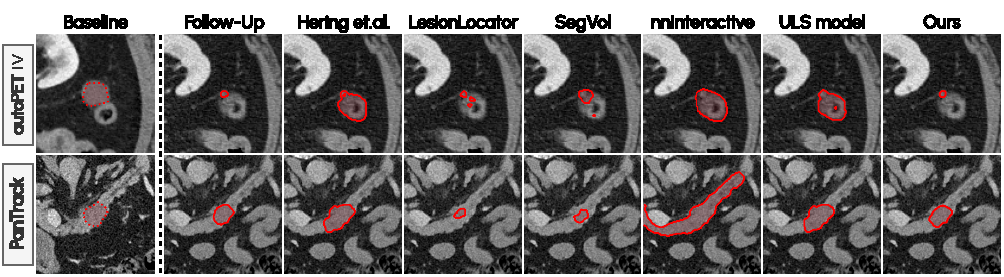
\includegraphics[width=1\textwidth]{figures/qualitative_all.pdf}
\vspace{-0.7cm}
\caption{\textbf{Qualitative comparison} on autoPET IV (top) and PanTrack (bottom). Single-timepoint baselines struggle with ambiguous lesion volumes. In the top row, a shrinking lesion borders the colon; without the baseline appearance as context, competing models fail to isolate the correct structure when prompted near the organ boundary.}
\label{fig:qualitative}
\end{figure}

% \noindent\textbf{OOD Generalization on PanTrack.} On PanTrack—originating from a different institution, scanner manufacturer, and pathology characterized by diffuse, fuzzy boundaries—our method maintains its superiority. Strikingly, our model's \textit{automatic} tracking performance on this unseen dataset (58.2 DSC) not only closely approaches its own verified performance (60.0 DSC), but outright surpasses the \textit{verified} performance of all competing foundation models (e.g., ULS at 53.4 DSC). This demonstrates that ``in the wild,'' our framework delivers highly reliable, fully automated tracking while natively preserving the safety of optional clinician refinement.

\noindent\textbf{OOD Generalization on PanTrack.} Despite PanTrack's different scanners, institutions, and fuzzy lesion boundaries, our method maintains its superiority. Strikingly, our model's \textit{automatic} tracking performance (58.2 DSC) not only closely approaches our \textit{verified} performance (60.0 DSC), but outright surpasses the \textit{verified} results of all competing models (e.g., ULS at 53.4 DSC). This proves our framework delivers highly reliable automated tracking "in the wild" while natively preserving the safety of optional clinician correction.